


\section{KDE Requirements Engineering}

Der folgende Teil beschreibt das Requirements Engineering bei dem Open Source
Projekt KDE. Ein Großteil der Informationen wurde der offiziellen
deutschsprachigen Website von KDE entnommen\cite{1}. 
%Quelle:https://de.kde.org/

\subsection{Requirement Engineering}
Requirements Engineering umfasst das Ermitteln, Analysieren, Spezifizieren und
Validieren aller Eigenschaften und Rahmenbedingungen eines Softwaresystems, die
über seinen gesamten Lebenszyklus gewünscht werden bzw. relevant sind\cite{2}.  
%Quelle:http://www.enzyklopaedie-der-wirtschaftsinformatik.de/lexikon/is-management/Systementwicklung/Hauptaktivitaten-der-Systementwicklung/Problemanalyse-/Requirements-Engineering/index.html

\subsection{Requirement Engineering in Open Source projekten}
Requirement Engineering bei Open Source Projekten unterscheidet sich von dem
gewöhnlicher Projekte(wie z.B. bei Firmen die als Dienstleister Software
entwickeln). Normalerweise werden die Anforderungen vom Kunden entgegen genommen
und zusammen mit dem Ersteller der Software zu realistischen und
aufgabenorientierten Requierements umformuliert. Doch bei Open Source Projekten
gilt es bestimmte Ziele zu erfüllen, wie das Endprodukt ausehen soll, dann
werden Requirements von der Community gegeben und von den Entwicklern erstellt.

%Quelle:

\subsection{Quellen für Requirements bei KDE}
Das Sammeln von Requirements bei KDE erfolgt über Benutzer Feedback,
Fehlerrückmeldungen und wirtschaftlichen Interessen. Feedback und Fehler werden
auf der Website über eine Adresse angenommen\cite{3}.
%http://bugs.kde.org 
%über das sammeln von requirements wegen wirtschaftlichen Interessen wurde
%nichts weiter? angegegben
% Quelle:https://techbase.kde.org/Development/Software_Engineering_Framework#Requirements_Gathering

\subsection{Dokumentation von KDE}
Die Dokumentation von KDE wird mit dem Produkt selbst ausgeliefert und dient
auch als hilfe Datei. Deswegen ist sie mehr als Handbuch bzw. als Hilfestellung
gedacht und weniger zum formulieren, festhalten oder entnehmen von Requirements.
Als Beispiel wird einem gezeigt wie man die Lautstärke für Ausgabegeräte
einstellt aber nicht welche Anforderungen an den Lautstärke Regler gestellt
wurden\cite{4}.

%Quelle:https://docs.kde.org/index.php?language=de&package=kdemultimedia
\subsection{Umgang mit Requirements bei KDE}
Die Arbeit an KDE verläuft ähnlich zu der bei Linux. Eine Aufgabe wird in
Teilaufgaben aufgeteilt, dann werden verantwortliche für diese Teilaufgaben
gesucht und denen die Teilaufgabe übertragen. Wodurch diese als Ansprechpartner
und Verantwortlicher dafür dienen. Als Beispiel kann man in folgendem Bild
KDEgames sehen.
%
\begin{figure}[h]
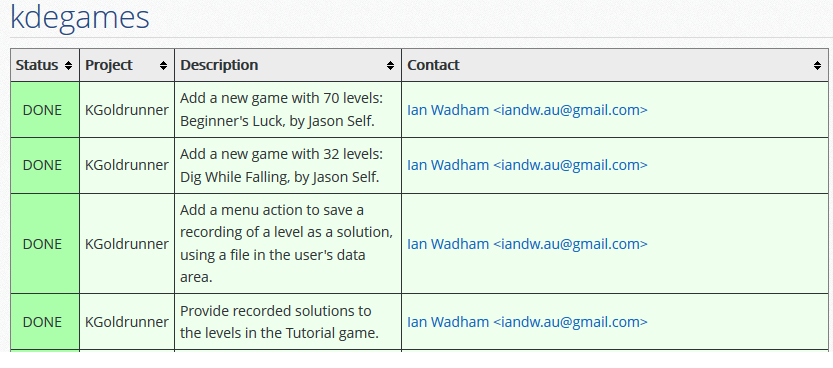
\includegraphics[width=\columnwidth]{images/KDE_games.png}
\caption{KDEgames\cite{5}}
\end{figure}
%Bild KDE Games
Das Bild zeigt einen Ausschnitt einer Tabelle die der Quelle, der KDE
Website entnommen wurde\cite{5}.
%Quelle:https://techbase.kde.org/Schedules/Applications/15.12_Feature_Plan
Die Tabelle hat vier Spalten. Die Erste zeigt den Status der Aufgabe an, DONE
IN PROGRESS oder TODO. Die zweite zeigt den Namen des Projekts. Die Dritte eine Beschreibung des Projekts und die vierte den Verantwortlichen für das Projekt.\\
Dadurch wird die Bearbeitung der einzelnen Projekte dokumentiert.

Besprochen werden die Requirements und andere Aufgabenspezifische teile über Mailinglisten. Damit werden Diskussionen und Absprachen durchgeführt.
Diese kann man ebenfalls über die Website einsehen, um einen Einblick in den
Verlauf eines Projekts zu erhalten.

Zusätzlich werden noch Requirements an bestimmte Teile des Produkts wie z.B.
Software die enthalten sein muss gestellt. Also um bei der KDE Auslieferung z.B.
bestimmte Networking Funktionen zu unterstützen benötigen wir rdesktop. Das
nachfolgende Bild zeigt ein Beispiel für Networking und Browsing.
\begin{figure}[h]
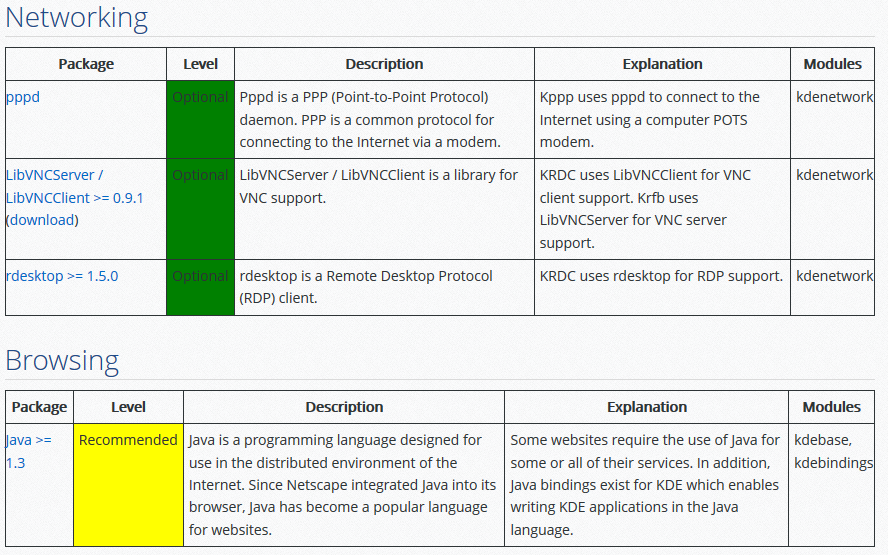
\includegraphics[width=\columnwidth]{images/KDE_Net_B.png}
\caption{Networking und Browsing\cite{6}}
\end{figure}
%network games req optional Contact
Das Bild zeigt zwei Tabellen die der Quelle, der KDE
Website entnommen wurden\cite{6}.
%Quelle:https://techbase.kde.org/Schedules/KDE4/4.4_Requirements
Die Tabellen haben jeweils 5 Spalten. Die erste Spalte enthält den Namen des
Packages das unter Umständen benötigt wird. Die zweite Spalte enthält das Level,
also wie stark die Funktion abhängig von dem Requirement ist, unterteilt in
Required, Recommended und Optional. Die dritte Spalte enthält eine Beschreibung
was dieses Package enthält und die vierte Spalte eine Erklärung warum dieses
Requirement für die Funktion nötig ist. In der fünften und letzten Spalte ist
festgehalten zu welchem Modul das Package gehört.

\subsection{Fazit}
Abschließend kann ich zum Requirements Engineering bei KDE sagen, dass das
Vorgehen mir schon zu Beginn meiner Nachforschung ähnlich zu dem vorkam, was ich
über das Vorgehen bei der Arbeit an Linux selbst erfahren habe. Das Aufteilen
der Aufgaben an verschiedene Personen die dann zuständig sind und stark dafür
verantwortlich die Requirements zu fassen bzw. zu bestimmen. Dies hat sich
auch beim Abschluss meiner Nachforschung bestätigt, weshalb ich dieses Vorgehen
im obrigen Teil auch wiedergegeben habe. Dieses Vorgehen ist für gewöhnliche
Projekte eher untypisch und unterschiedet sich auch von den klassischen Methoden
die in der Vorlesung aufgeführt wurden. %Für Open Source Projekte ist zwar ein
%anderes Vorgehen erfordlich aber es hätte bestimmt auch eine andere Möglichkeit
%gegeben.
Wobei dazuzusagen ist, dass KDE ein Open Source Projekt ist und deswegen eine
andere Vorgehensweise erfordert und es genauso seine Berechtigung hat, den KDE
und Linux sind beide erfolgreiche Projekte.
%untypisches requirement Engineering kein normales
%aufsteleln typisch linux / Open Source?
%two Bilder ..
%Linux typisch guru
\begin{thebibliography}{x}
   \bibitem[1]{1}'https://de.kde.org/'
   \bibitem[2]{2}'http://www.enzyklopaedie-der-wirtschaftsinformatik.de/lexikon/is-management/Systementwicklung/Hauptaktivitaten-der-Systementwicklung/Problemanalyse-/Requirements-Engineering/index.html'
   \bibitem[3]{3}'https://techbase.kde.org/Development/Software\_Engineering\_Framework\#Requirements\_Gathering'
   \bibitem[4]{4}'https://docs.kde.org/index.php?language=de\&package=kdemultimedia'
   \bibitem[5]{5}'https://techbase.kde.org/Schedules/Applications/15.12\_Feature\_Plan'
   \bibitem[6]{6}'https://techbase.kde.org/Schedules/KDE4/4.4\_Requirements'
\end{thebibliography}


